%% LaTeX2e class for student theses
%% sections/proposal.tex
%% 
%% Karlsruhe Institute of Technology
%% Institute for Program Structures and Data Organization
%% Chair for Software Design and Quality (SDQ)
%%
%% Dr.-Ing. Erik Burger
%% burger@kit.edu
%%
%% Version 1.3.6, 2022-09-28

\chapter{Secure Computation Platform Blueprint}
\label{ch:proposal}

\section{Trust Model}
\label{sec:trust-model}

\todo[inline]{Explain needed services}

\subsection{Chain of Trust}

\subsection{Roles}

\subsubsection*{Infrastructure Provider}

The infrastructure provider is responsible for the availability of the
infrastructure used to provide compute, networking, and storage resources. As
such the infrastructure controls and has access to the physical hardware and
firmware.

\subsubsection*{Service Provider}

The service provider is responsible for managing services that utilize the
infrastructure provided by the infrastructure provider in order to ease the
development and deployment of workloads. As such the service provider is not
only responsible for deploying the applications, but also to provide services
that allow the retrieval of attestation evidence and initialize TEE
environments.

It may be the case that the service and infrastructure provider roles are
aggregated into the same entity. As the attestation evidence is produced and
signed by the hardware vendor grouping these two roles does not affect the trust
model.

\subsubsection*{Application Owner}

The application owner designs and implements application workloads that will be
deployed and orchestrated by the service provider. This role needs to prove to
the customer aspects of compliance to the defined requirements. As such the
application owner has to provide TEE initialization images and attestation
verification services, or designate a trusted party to do so.

The application owner and service provider role should not be taken on by the
same entity, as the verification of the TEE provided by the service provider is
a responsibility of the application owner. Otherwise, the attestation results
can not be trusted.

\subsubsection*{Data Owner}

As the owner of the data used and manipulated by the application, this role is
concerned with the visibility, integrity of their data and the compliance of the
application with the requested requirements.

\section{Architecture}
\label{sec:proposal:architecture}

\subsection{Design Choices}

\subsubsection*{PaaS Service Model and Containers}

\begin{table}
  \centering
  \footnotesize
  \setitemize{noitemsep,topsep=0pt,leftmargin=*}
  \scalebox{0.9}{\begin{tabular}{L{70pt}|L{100pt}L{100pt}L{100pt}}
                                                     & \multicolumn{1}{C{100pt}}{IaaS} & \multicolumn{2}{c}{PaaS}                                                                   \\
                                                     &                                 & \multicolumn{1}{c}{Container}                             & \multicolumn{1}{c}{Binary}     \\
  \hline
  \hline
  Provides                                           & VMs with CC enabled             & Container runtime that runs containers in a CC enabled VM & CC enabled runtime environment \\
  \hline
  Infrastructure \& Orchestration managed by         & Application Owner
                                                     & Service Provider                &
  Service Provider                                                                                                                                                                  \\
  \hline
  Development Environment managed by                 & Application Owner               & Application Owner                                         & Service Provider               \\
  \hline
  Notes                                              &
  \begin{itemize}
    \item Everything has to be managed by
          the application owner
    \item Goal is to reduce complexity
  \end{itemize}              &
  \begin{itemize}
    \item Big attack surface (TCB) if done
          bad
    \item Much more in control of the service provider
    \item Services supporting CC usage can be
          provided by the service provider
  \end{itemize} &
  \begin{itemize}
    \item Least control by application owner
    \item Either complex dependency management
          and language support by the service provider
    \item Or language or dependency limitations
  \end{itemize}                                                                                                                                       \\
\end{tabular}
}
  \caption{An overview over different services models.}
  \label{table:service-models}
\end{table}

\todo[inline]{Outsource table, for use as an image}

In order to align with goal \subGoalRef{1}{1} this proposal will focus on the
PaaS service model. The management of the infrastructure is abstracted in the
form of services that are provided to the client as a platform.

Containers resolve the issue of dependency management for the service provider
by allowing application owners to package all-in-one application images that can
be developed and deployed with the help the provided services (goal
\subGoalRef{1}{2}).

See table \ref{table:service-models} for a comparison between the IaaS, PaaS
with binary applications, and PaaS with container applications service models.

\subsubsection*{Kubernetes}

As a base for the platform this proposal will utilize Kubernetes which will
provide basic platform features common to PaaS offerings. This allows us to
focus on the confidentiality part (goal \goalRef{2}) of this thesis by extending
and replacing components in the Kubernetes architecture.

In section \ref{sec:kubernetes-platform-base} we discussed different ways to
implement confidentiality in Kubernetes. While applying confidentiality on a
node or container level, node level confidentiality introduces challenges around
limiting privileges of cluster administrators and container level
confidentiality conflicts with the Kubernetes design of pods. For these reasons
pod level confidentiality makes the most sense in the context of achieving goal
\goalRef{2} in a Kubernetes context.

There is a project dedicated on implementing pod level confidentiality into a
Kubernetes cluster which aligns with our goals. The Confidential Containers
project\footnote{https://github.com/confidential-containers} wants to separate
the service provider from the guest applications trust model, allow application
owners to enforce security requirements, apply least privilege principles to the
Kubernetes cluster administrator capabilities (\subGoalRef{2}{1}), enable
transparent deployment of unmodified containers (\subGoalRef{2}{2}), and support
multiple TEE implementations on various hardware platforms. The following
architecture will be largely based on this projects' effort, summarizing the
current state of the project, gather problems that still need to be solved and
their corresponding solution proposals.

\subsubsection*{VM-based TEEs}

\todo[inline]{Process-based TEEs similar utilizing libOSes}

\subsection{Overview}

\begin{figure}
  \centering
  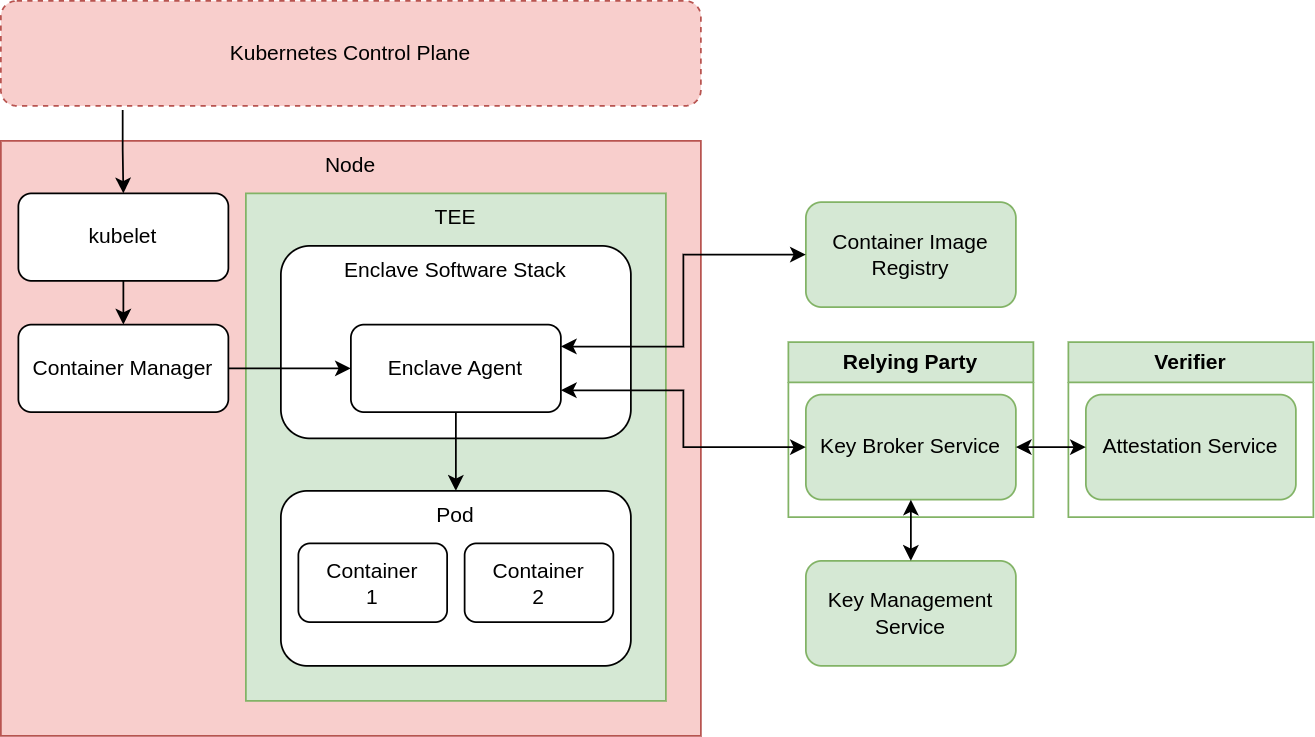
\includegraphics[width=\linewidth]{resources/confidential-containers-overview.png}
  \caption[A simplified overview over the Confidential Containers architecture]{
    Entities and Components marked in red are untrusted, while those marked in
    green are trusted.
  }
  \label{fig:confidential-containers-overview}
\end{figure}

The roles defined in this architecture are based on RATS. While we introduced
RATS in section \ref{sec:rats} we will go deeper into the architecture in the
next section.

Figure \ref{fig:confidential-containers-overview} shows a brief overview over
the Confidential Containers architecture. In order to protect pods, 

\subsection{Remote Attestation}

\todo[inline]{Deep dive into RATS architecture}

\subsection{Kata Containers}

\todo[inline]{Enclave agent responsible for communicating with container manager}
\todo[inline]{Enclave Software Stack includes ...}
\todo[inline]{Measured and part of the evidence}

\subsection{Control Plane Security}

\todo[inline]{Remove privileged commands from untrusted control plane}
https://github.com/confidential-containers/community/issues/53

\subsection{Networking}

\subsection{Storage}

\todo[inline]{Ongoing work}
https://github.com/confidential-containers/documentation/issues/39
